
\documentclass[a0,portrait]{a0poster}

\usepackage{multicol} % This is so we can have multiple columns of text side-by-side
\columnsep=100pt % This is the amount of white space between the columns in the poster
\columnseprule=3pt % This is the thickness of the black line between the columns in the poster

\usepackage[svgnames]{xcolor} % Specify colors by their 'svgnames', for a full list of all colors available see here: http://www.latextemplates.com/svgnames-colors

\usepackage{times} % Use the times font
%\usepackage{palatino} % Uncomment to use the Palatino font

\usepackage{graphicx} % Required for including images
\graphicspath{{figures/}} % Location of the graphics files
\usepackage{booktabs} % Top and bottom rules for table
\usepackage[font=small,labelfont=bf]{caption} % Required for specifying captions to tables and figures
\usepackage{amsfonts, amsmath, amsthm, amssymb} % For math fonts, symbols and environments
\usepackage{wrapfig} % Allows wrapping text around tables and figures
\usepackage{tikz}
\usepackage{subfigure}
\begin{document}

%----------------------------------------------------------------------------------------
%	POSTER HEADER 
%----------------------------------------------------------------------------------------

% The header is divided into two boxes:
% The first is 75% wide and houses the title, subtitle, names, university/organization and contact information
% The second is 25% wide and houses a logo for your university/organization or a photo of you
% The widths of these boxes can be easily edited to accommodate your content as you see fit

\begin{minipage}[b]{1\linewidth}
\centering \veryHuge \color{Black} \textbf{Inventarios forestales a través del procesamiento de imágenes}\\ % Title
\huge \textbf{José Angel Ramírez Cantú \& Satu Elisa Schaeffer}\\[0.5cm] % Author(s)
\huge Facultad de Ingeniería Mecánica y Eléctrica\\[0.4cm] % University/organization
\Large \texttt{jose.ramirezcnt@uanl.edu.mx}\\
\end{minipage}
%
\begin{minipage}[b]{0.25\linewidth}
\vspace*{-70mm}
\hspace*{15mm}

\includegraphics[width=12cm]{uanl.png}\hspace*{480mm}
\includegraphics[width=10cm]{fime.jpg}
\end{minipage}

\vspace{1cm} % A bit of extra whitespace between the header and poster content

%----------------------------------------------------------------------------------------

\begin{multicols}{2} % This is how many columns your poster will be broken into, a portrait poster is generally split into 2 columns

%----------------------------------------------------------------------------------------
%	INTRODUCTION
%----------------------------------------------------------------------------------------

\color{Black} % SaddleBrown color for the introduction

\section*{Introducción}
El \emph{aprendizaje máquina}\footnote{Campo de la inteligencia artificial que desarrolla algoritmos capaces de aprender por medio de información.} es precisamente uno de los campos de la \emph{inteligencia artificial}\footnote{Ciencia encargada de desarrollar algoritmos capaces de imitar capacidades humanas.} que permite resolver esta clase de problemas, ya que gracias al aprendizaje supervisado se pueden usar técnicas de agrupamiento para clasificar distintas especies de árboles por medio de muestras recolectadas. En análisis de recorridos por drones, el enfoque está dirigido al área forestal dado que se puede utilizar el aprendizaje máquina para la gestión del inventario forestal, ayudando a reducir el fallo humano y optimizando las tareas de clasificación de especies arbóreas.

%----------------------------------------------------------------------------------------
%	OBJECTIVES
%----------------------------------------------------------------------------------------

\section*{Motivación}
Pese a que ya existen mecanismos de detección de objetos, muchos de ellos no funcionan con la precisión o la meta que deseamos, puesto que no se enfocan en un objetivo en particular, más sin embargo, la investigación se enfoca puramente en la detección de especies arbóreas (\emph{Abies, Encino y Pino}) utilizando muestras recolectadas en las zonas del Cilantrillo y Trinidad.
%----------------------------------------------------------------------------------------
%	MATERIALS AND METHODS
%----------------------------------------------------------------------------------------

\section*{Hipótesis}
Se sabe que el procesamiento de imágenes tiene como finalidad enfocarse en la búsqueda de un elemento en particular, las especies arbóreas (presente trabajo). Se plantea demostrar que el procesamiento de imágenes permitiría reducir tiempos de recorrido a pie y optimizar costos en cuanto a la realización de inventarios forestales por medio de técnicas tradicionales.


\section*{Objetivos}
El \textbf{objetivo} de realizar el inventario forestal por medio del procesamiento de
imágenes tiene un propósito más práctico que técnico. El algoritmo permitiría a quienes se encarguen de analizar las zonas forestales, reducir el tiempo invertido en aplicar técnicas tradicionales por técnicas de procesamiento de imágenes.\\

Estas técnicas  basadas en el aprendizaje máquina, las cuales van permitir
generar un inventario forestal mediante el recorrido de un dron y a su vez, analizarlo por medio de la inteligencia artificial con la finalidad de indicar las cantidad de especies reconocidas sobre una zona.
\subsection*{Objetivos específicos}
\begin{itemize}
\item Realizar un algoritmo capaz de detectar específicamente los árboles y su especie arbórea.
\end{itemize}

\begin{itemize}
\item El algoritmo debe extraer la información de un conjunto de especies arbóreas, mismas que servirían como modelo para una fase posterior de detección de especies arbóreas.
\end{itemize}

\begin{itemize}
\item El algoritmo debe ser capaz de detectar por si mismo las especies encontradas en cada una de las muestras recolectadas.
\end{itemize}

\section*{Descriptores de características globales}
Son los criterios que determinan la información más relevante al momento analizar cada imagen
\begin{description}

\item[Color]{Utiliza un histograma para determinar la intensidad de un color en un pixel.}\\

\hspace*{50mm}\includegraphics[width=0.15\textwidth]{6100.jpg}
   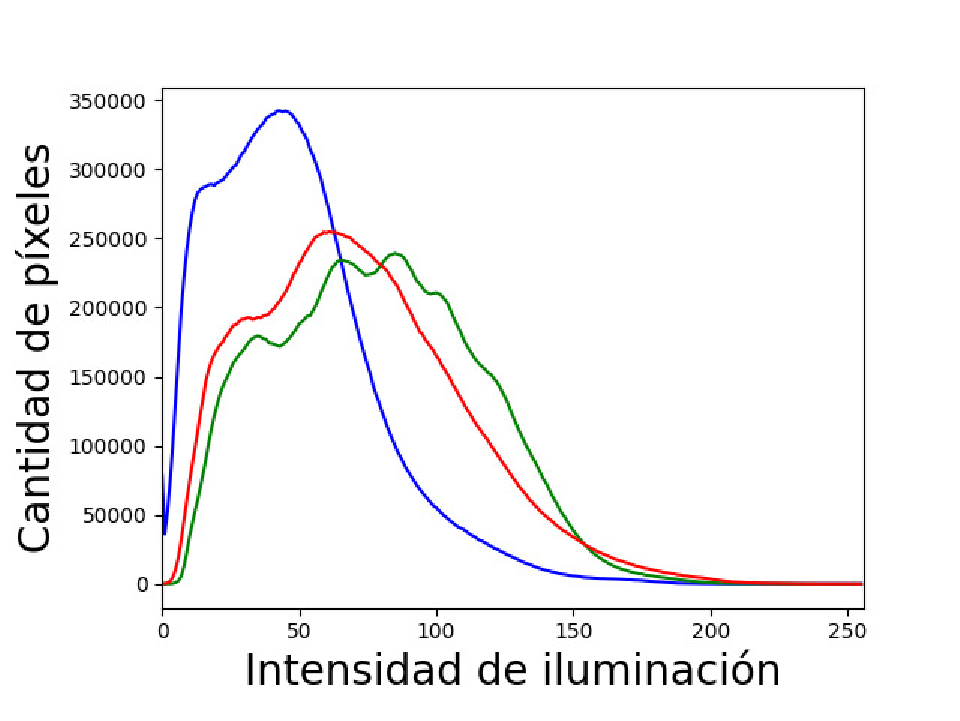
\includegraphics[width=0.15\textwidth]{histograma.pdf}
\item[Forma]{Determina los pesos promedio de la intensidad de píxel sobre una imagen.}\\

   \hspace*{80mm}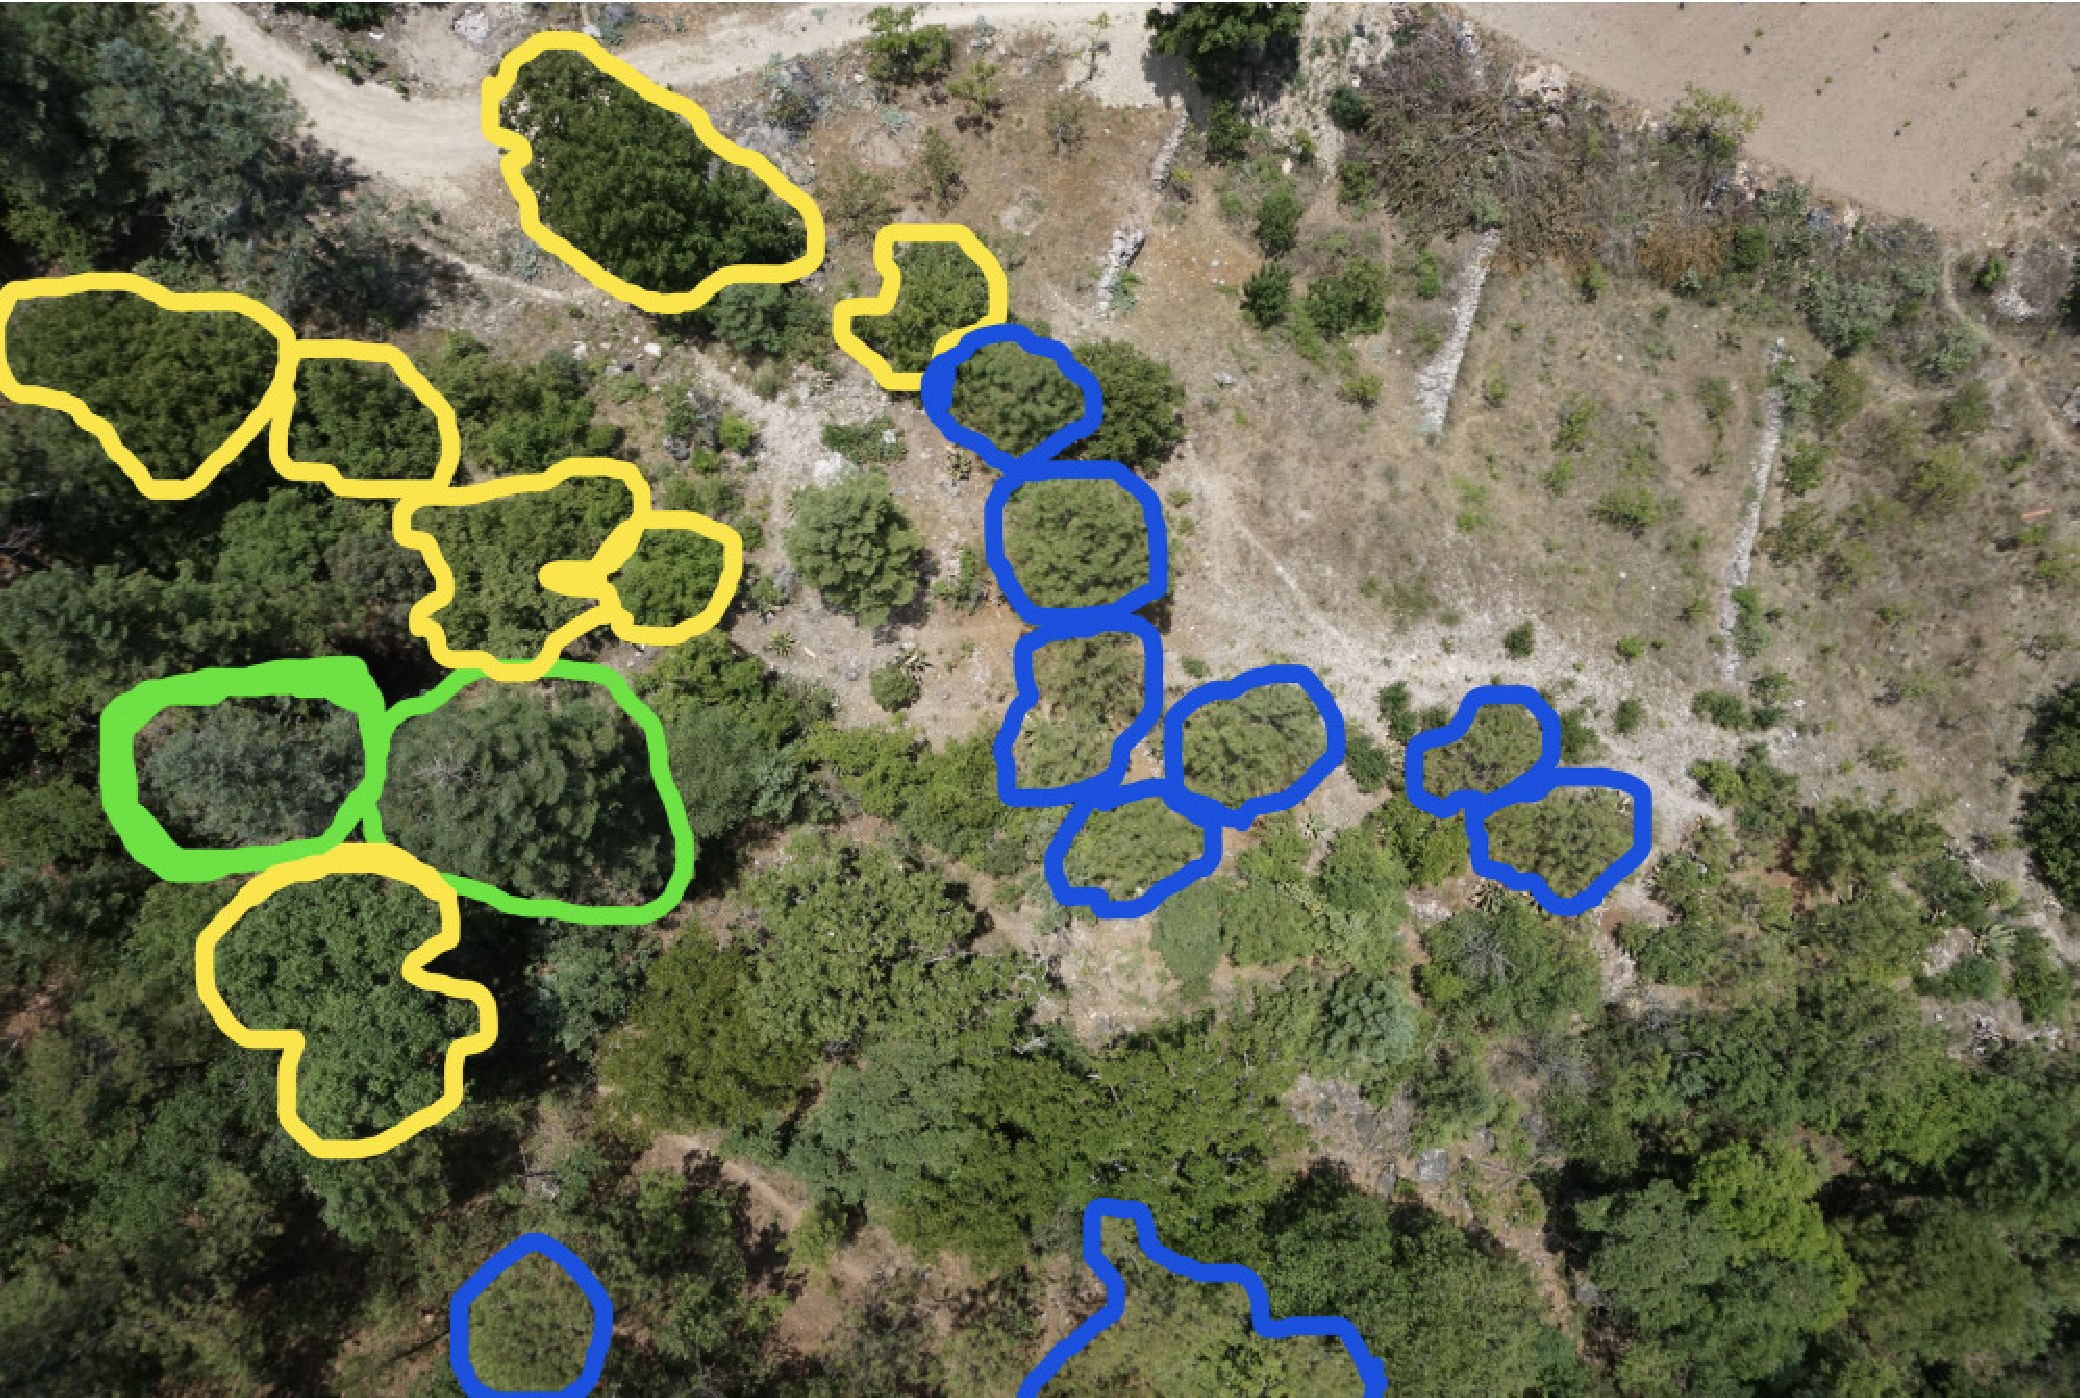
\includegraphics[width=0.15\textwidth]{Anotaciones-ex.pdf}
   
\item[Textura]{Identifica el patrón de las hojas que están sobre un árbol.}\\

\hspace*{25mm}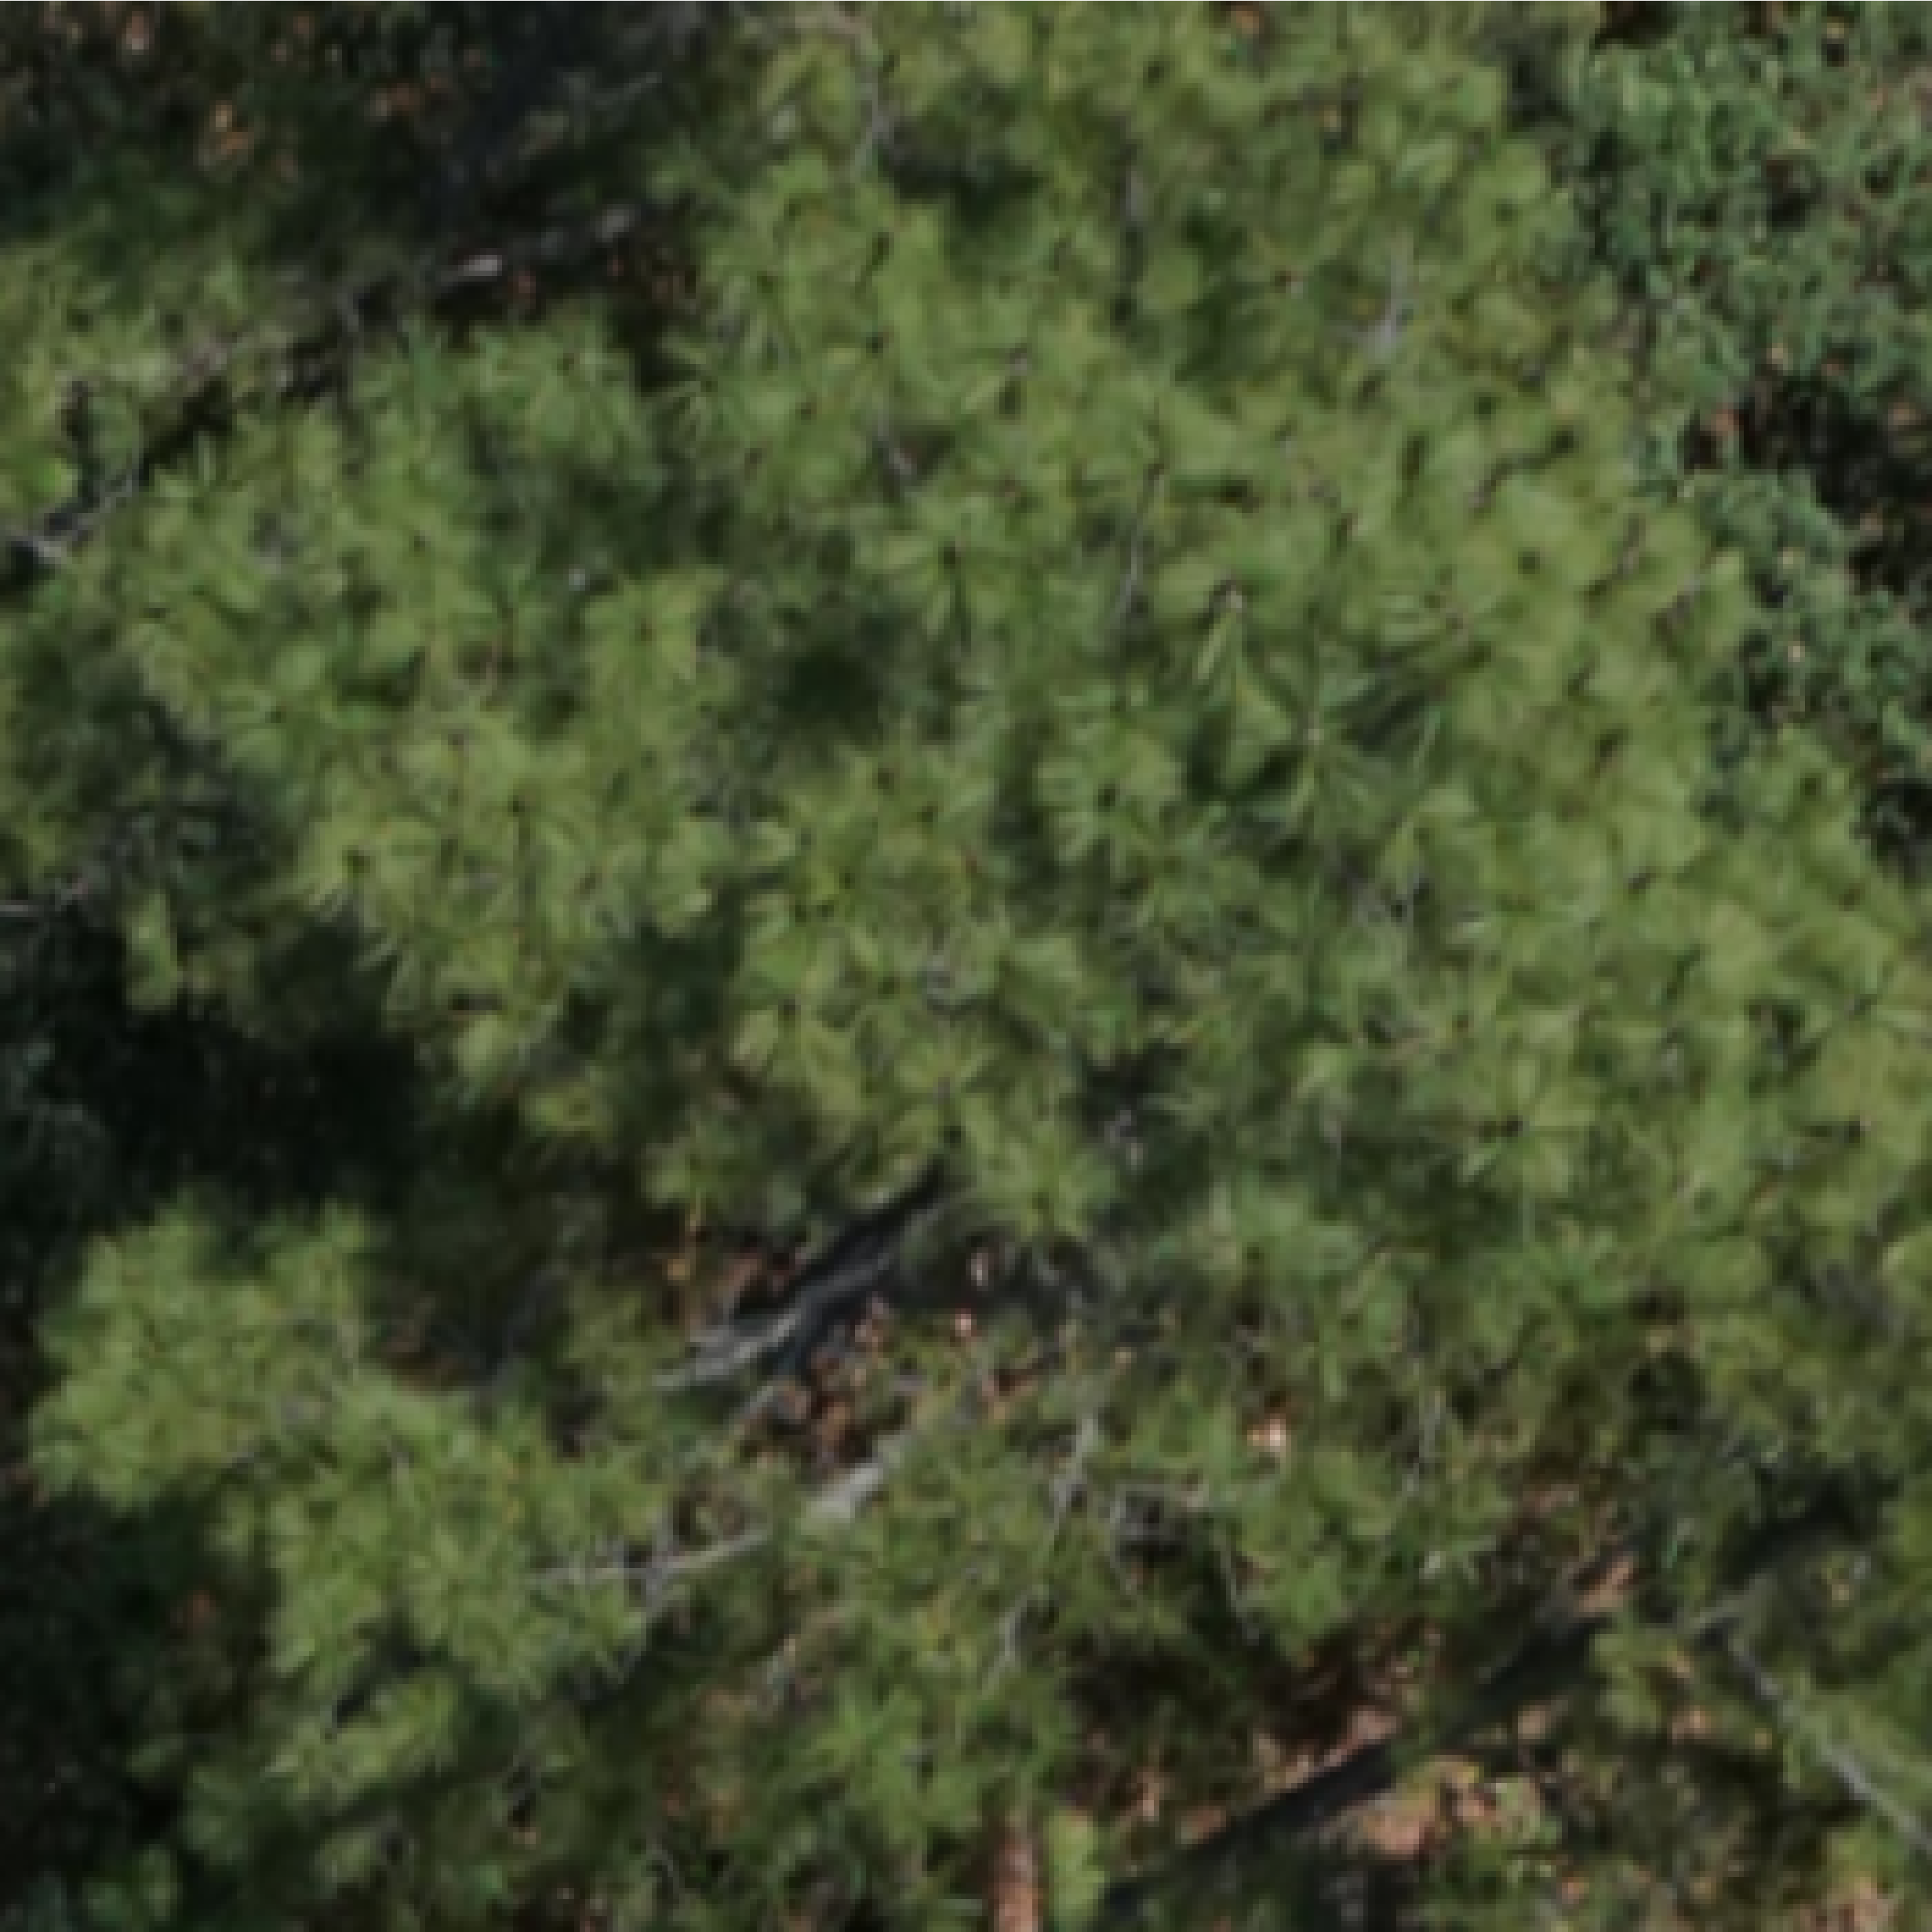
\includegraphics[width=0.10\textwidth]{1_res.pdf}
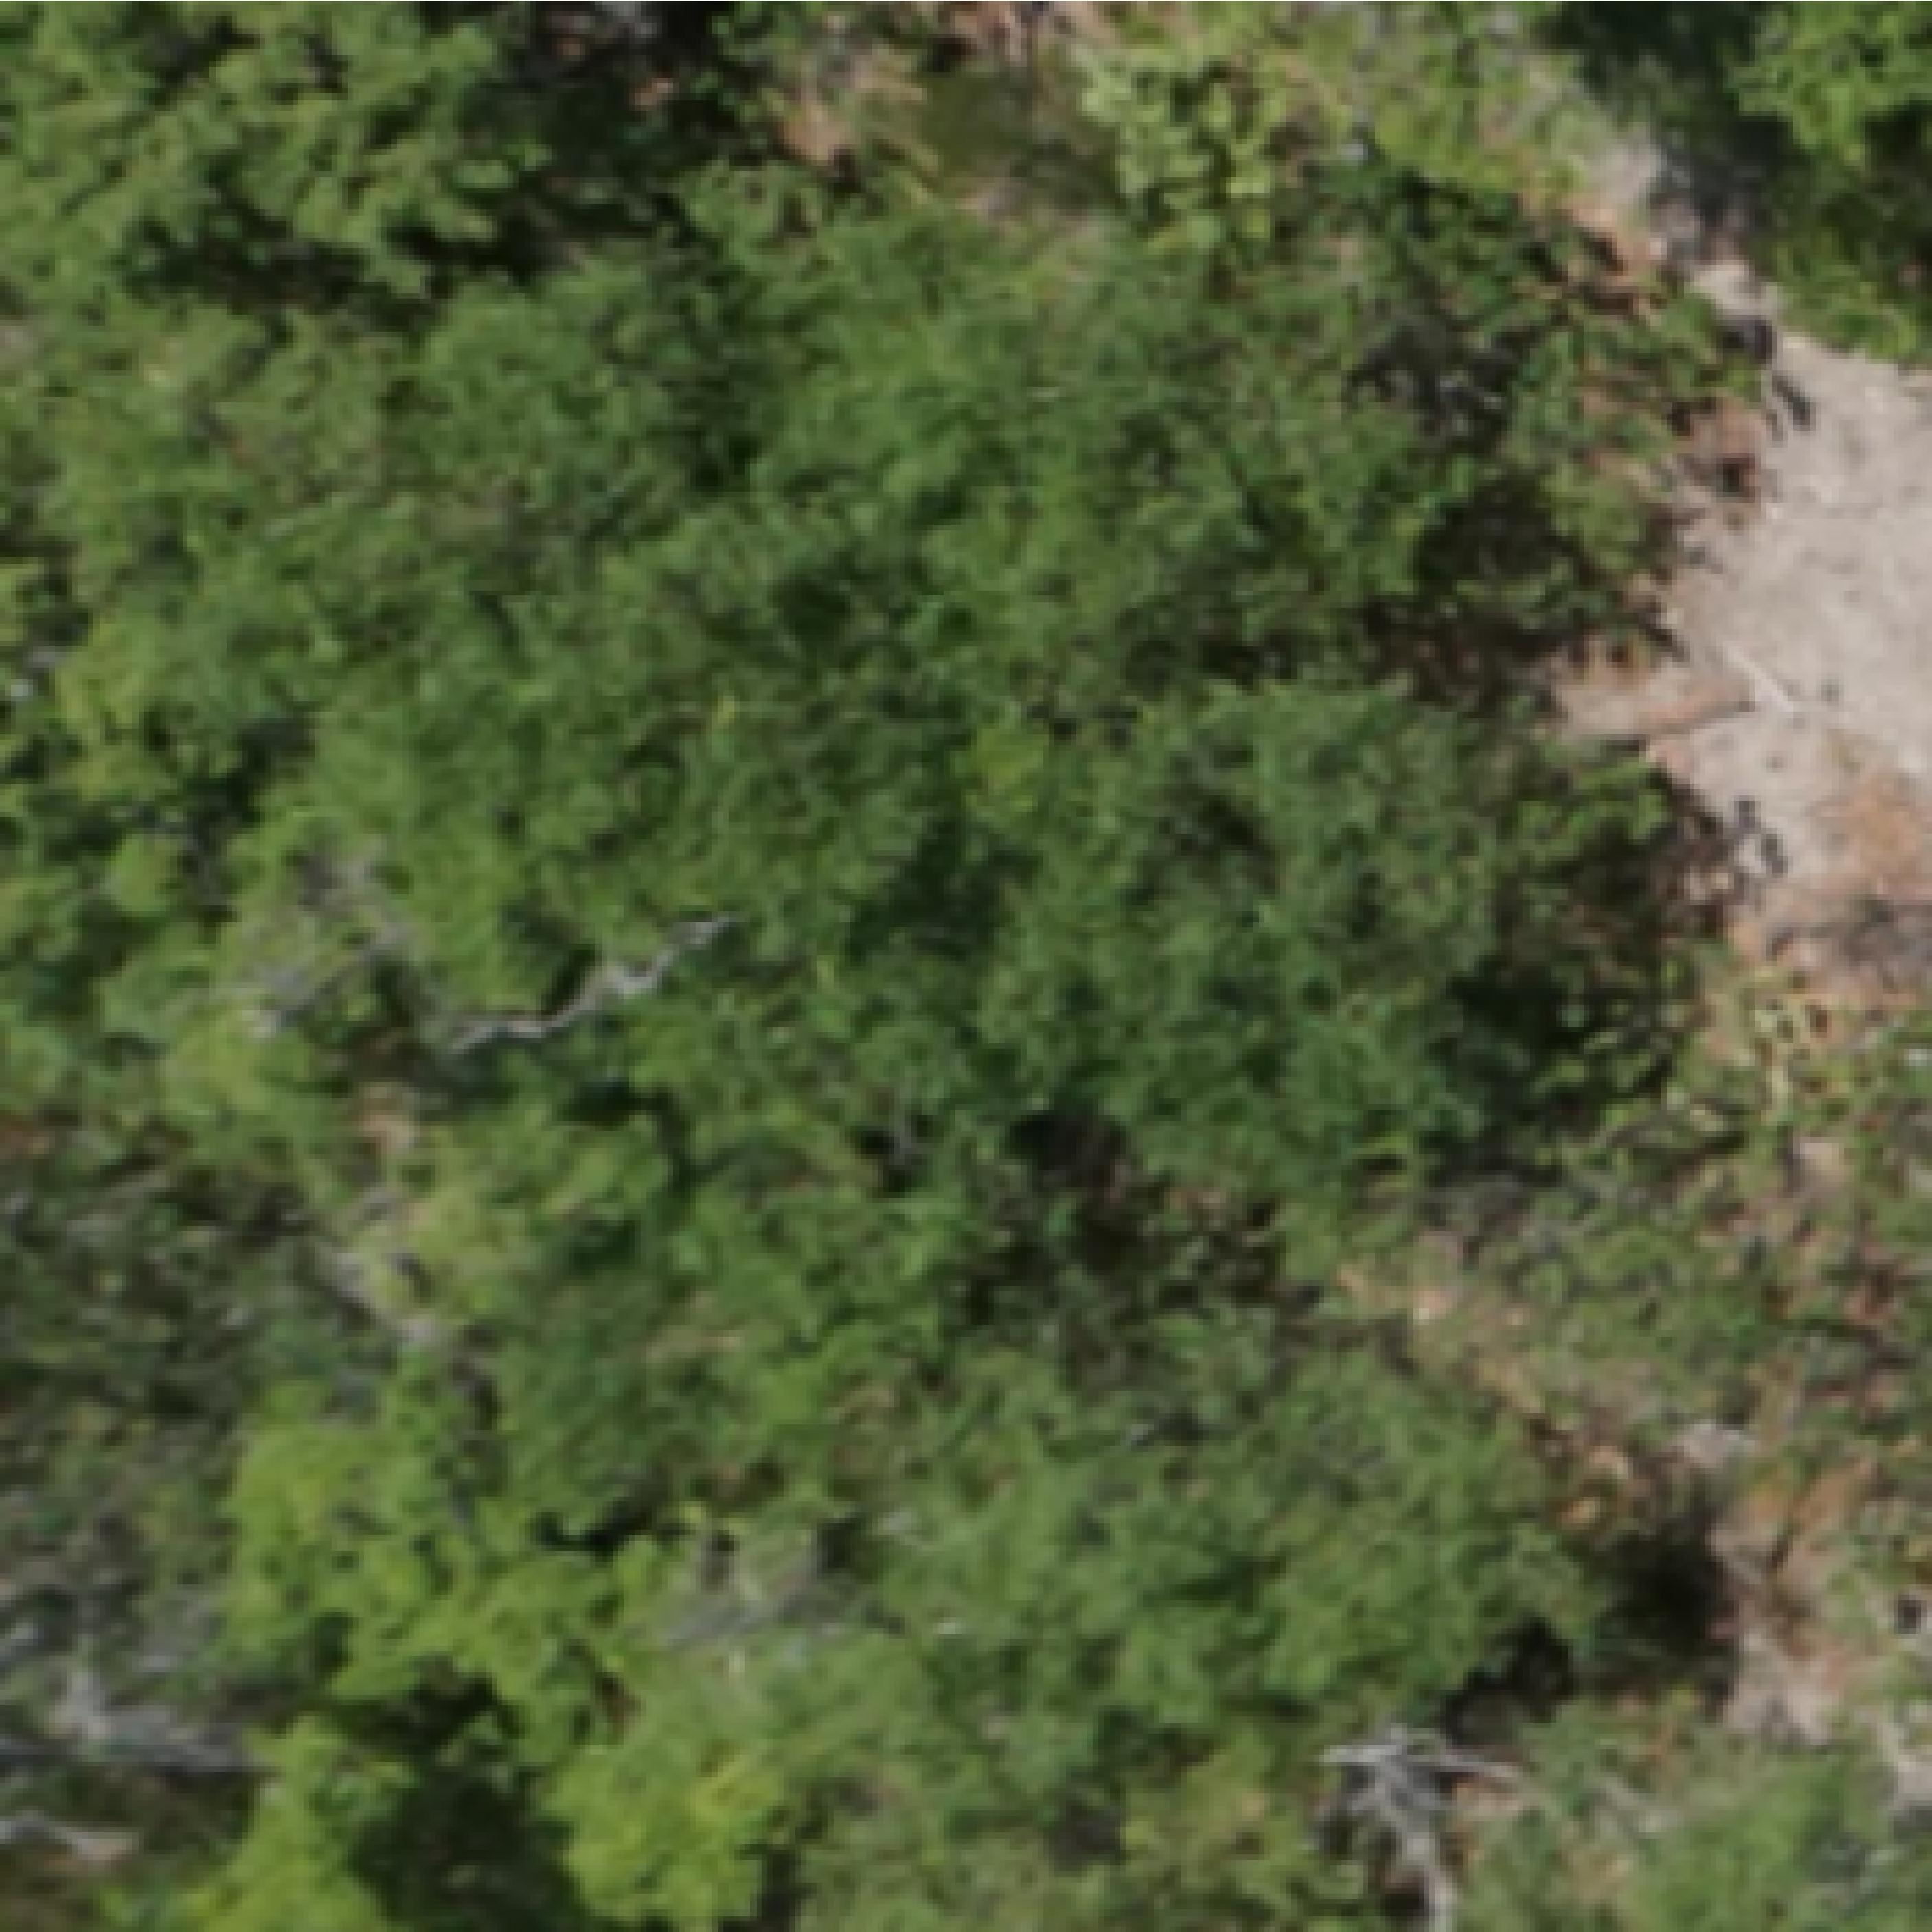
\includegraphics[width=0.10\textwidth]{2_res.pdf}
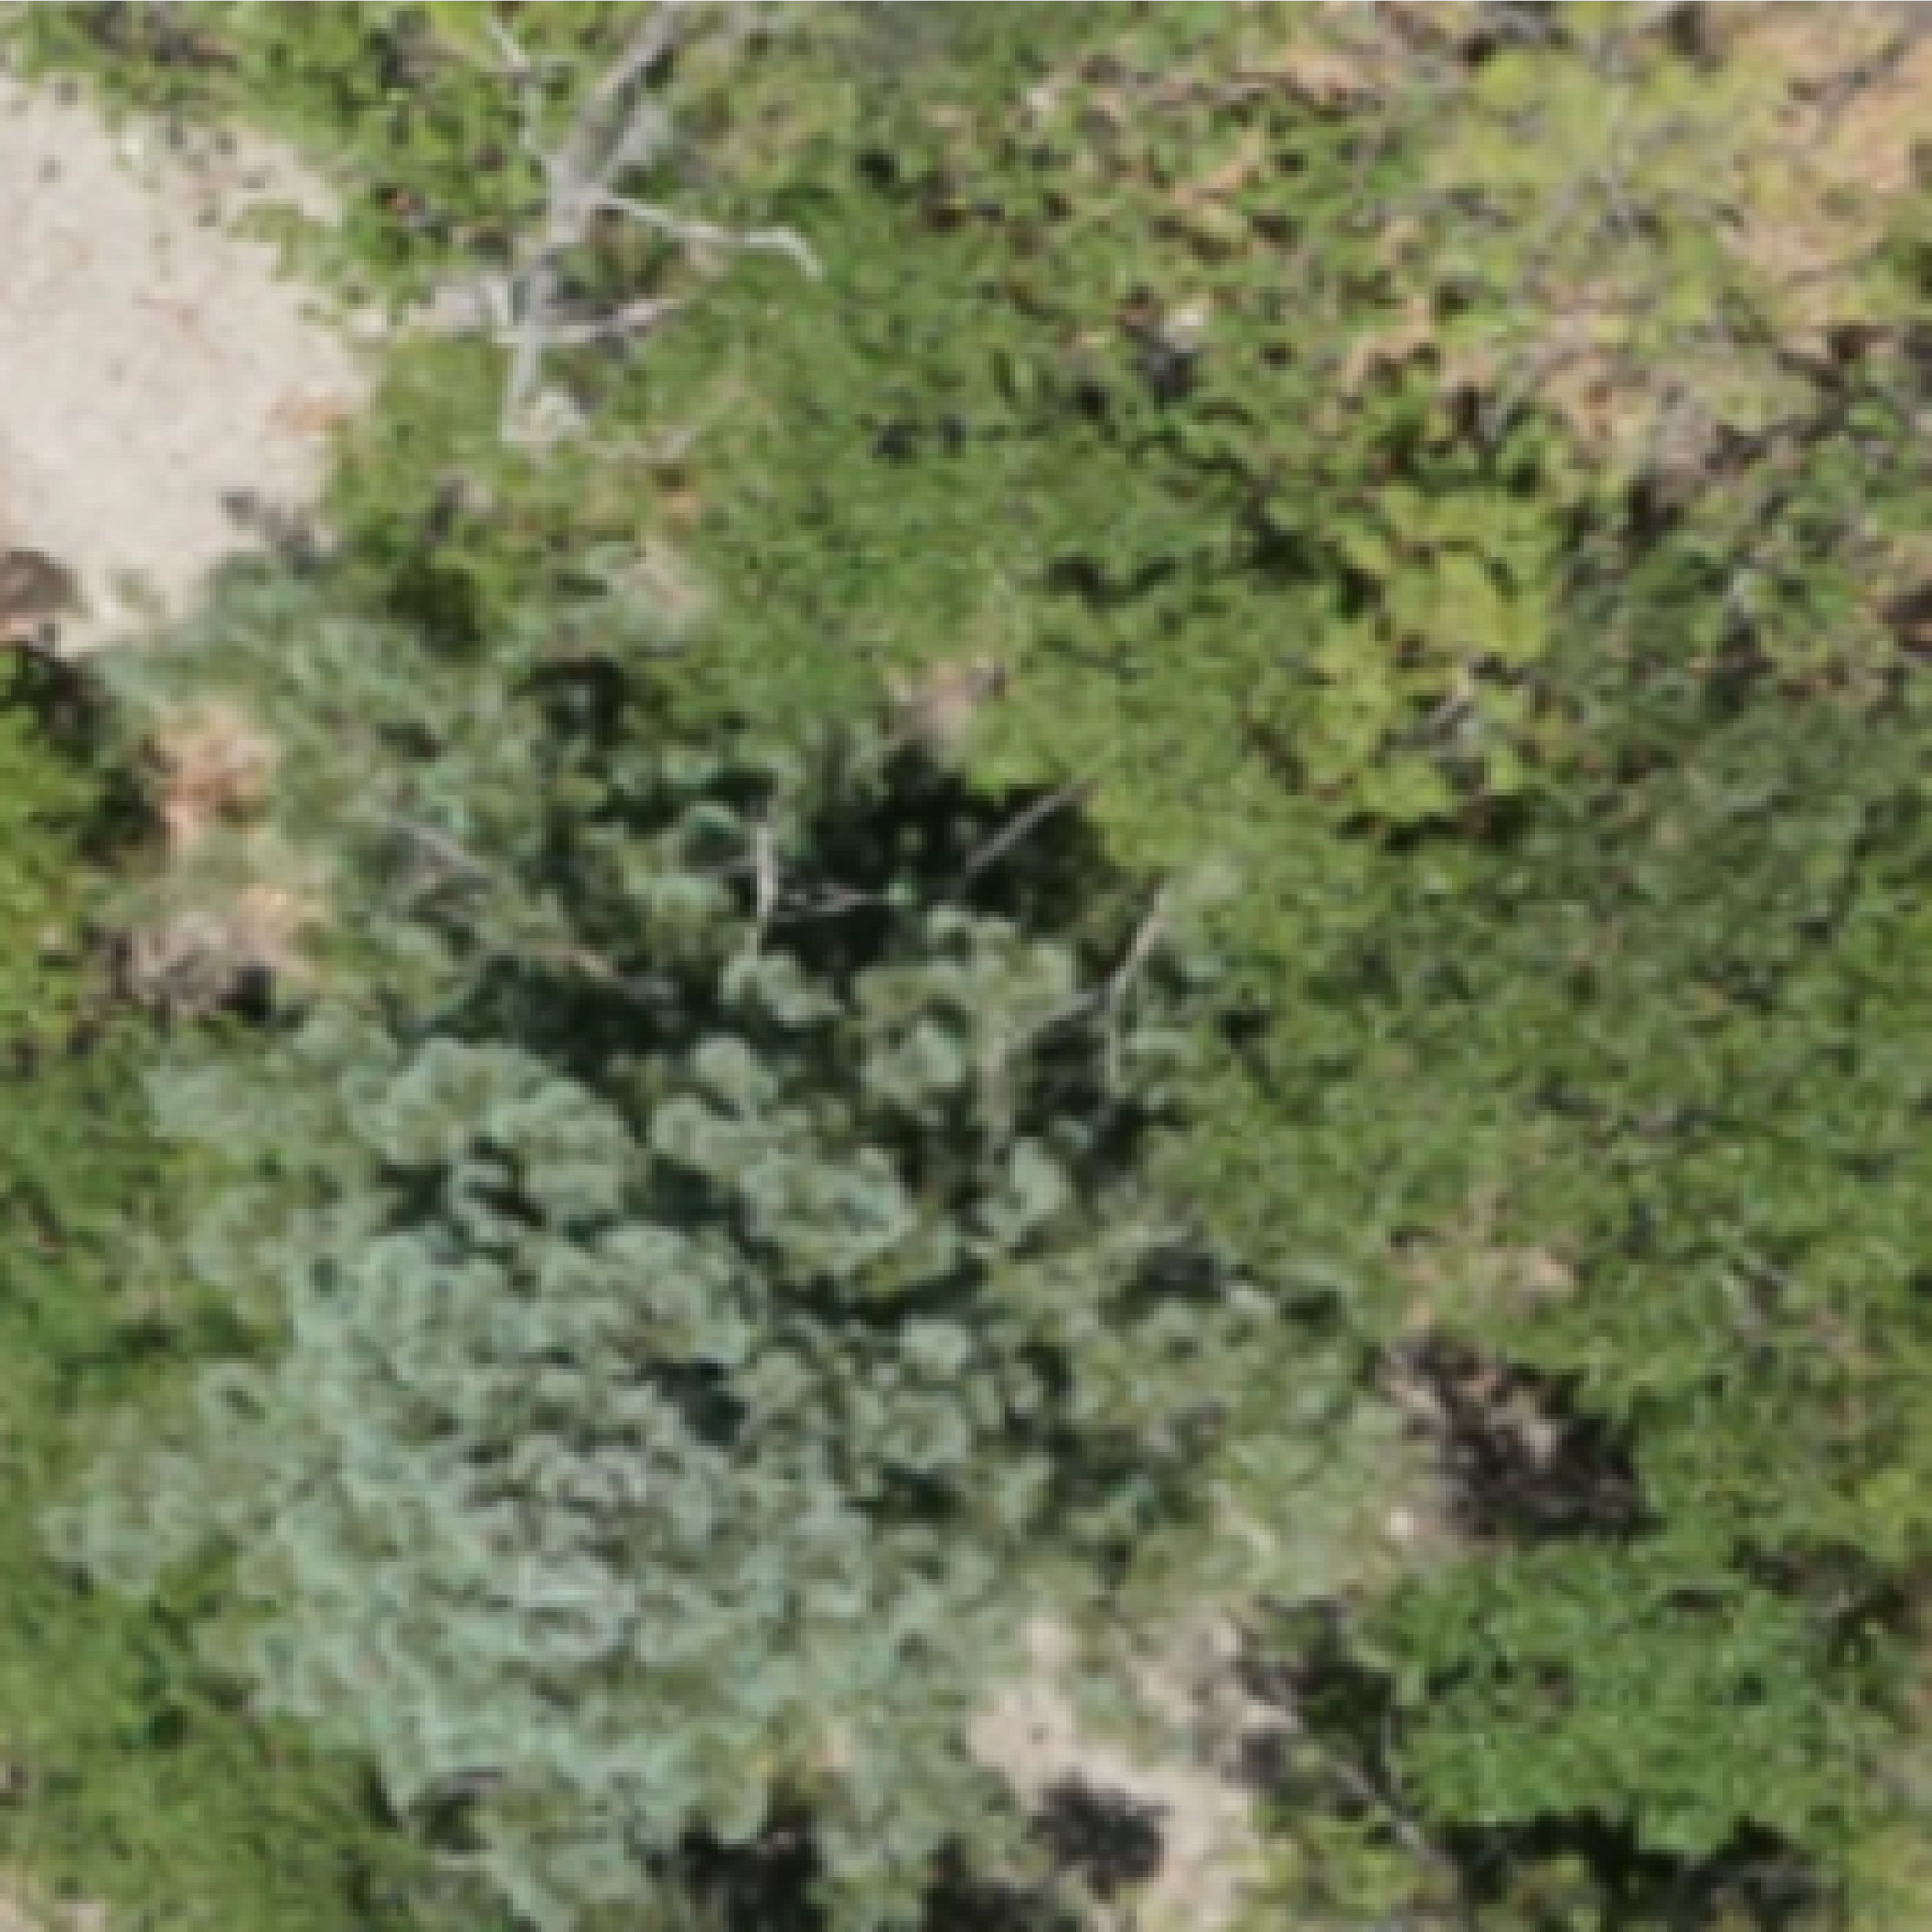
\includegraphics[width=0.10\textwidth]{3_res.pdf}\\
\hspace*{50mm}(a) Encino \hspace*{40mm} (b) Pino \hspace*{30mm} (c) Abies
\end{description}

\section*{Descriptores de características locales}
Estas cuantifican globalmente una imagen, sin embargo, para poder determinar las características que cuantifican localmente las regiones de una imagen es necesario determinar que descriptor es el mejor para describir los puntos de interés de una imagen completa o los puntos de interés de cierta región de la imagen.
\bigskip
\begin{description}
\item[Escalamiento:]{Transforma los datos de las características en rangos específicos de cero a uno.}
\item[Normalización:]{Desplaza y re-escala valores para alcanzar un rango entre cero y uno.}

\item[Escala invariante (SIFT):]{Extrae la información y adecua en comparaciones.}

\item[Acelarado robusto (SURF):]{Toma un vecino al rededor del punto seleccionado en la imagen y es dividido en sub-regiones para cada sub-región.}

\item[Característica de diferencias en forma de cadena binaria (BRIEF):]{Orientación y menor numero de diferencias a su alrededor.}

\item[ORB* rotada y orientada rápida:]{Determina estos puntos clave de una imágen.}
\end{description}
\vspace*{-15mm}
\section*{Solución propuesta}
\begin{description}
\item[Fase de recolección de muestras]{Se recolectan la muestras que serán utilizadas en fases posteriores.}

\item[Fase de procesamiento  de muestras]{Se modifican las muestras para únicamente dejar las muestras con información útil en fases posteriores.}\\
\hspace*{60mm}\includegraphics[width=0.15\textwidth]{DSC06080.pdf}  \includegraphics[width=0.15\textwidth]{DSC06080-sf-2.pdf}
\item[Fase de entrenamiento]{Se genera un modelo con las muestras obtenidas en la fase de procesamiento con la información recolectada de cada especie.}

\item[Fase de detección]{El modelo generado previamente en la fase de entrenamiento es utilizado para identificar y clasificar cada especie sobre una muestra útil.}
\item[Fase de combinación]{La muestra útil con las especies clasificadas en la fase de detección es combinada con la muestra original para poder determinar cuales muestras fueron detectadas sobre cada parte del sector forestal.}\\
  \hspace*{120mm}\includegraphics[width=0.15\textwidth]{result_combination.pdf}
\end{description}
\vspace*{-25mm}
\section*{Resultados}
\begin{description}
\item[Experimento $A$: Misma cantidad de especies por tamaño de clase.]{Toma la misma cantidad de muestras para cada clase.}

\item[Experimento $B$:  Cantidad total de especies por tamaño de clase.]{Toma todas las especies disponibles en cada clase.}

\item[Experimento $C$: Misma cantidad de especies utilizando espejos de muestras.]{Utiliza espejos de las muestras recolectadas en las clases que tengan una cantidad de muestras inferior al de la clase con más muestras para tener el mismo tamaño de muestras en todas las clases.}

\item[Experimento $D$: Umbralización.]{Compara tres niveles distintos de umbral  (0.15\%, 0.25\%, 0.50\%) para comparar el que mejor resultados proporciona.} 

\item[Experimento $E$: Límite de píxeles ausentes.]{Utiliza tres porcentajes de píxeles ausentes (0.75\%, 0.80\% y 0.85\%) para determinar la mayor cantidad de especies posibles en una muestra.}
\end{description}

\begin{center}
\begin{tabular}{|c|c|c|c|}
			\hline
			 \textbf{Experimento} & \textbf{Pino} & \textbf{Encino} & \textbf{Abies}\\
			\hline
			Experimento A & 67.3 & 18.4 & 14.4\\
			\hline
			Experimento B & 50.2 & 41.6 & 8.2\\
			\hline
			Experimento C & 58.1 & 34.3 & 7.7\\
			\hline
			Experimento D (0.75) & 66 & 17 & 17\\
			\hline
			Experimento D (0.80) & 62 & 24 & 14\\
			\hline
			Experimento D (0.85) & 18 & 15 & 18\\
			\hline
			Experimento E (0.75) & 70 & 20 & 10\\
			\hline
			Experimento E (0.80) & 63 & 25 & 12\\
			\hline
			Experimento E (0.85) & 66 & 22 & 12\\
			\hline
		\end{tabular}
\end{center}

\vspace*{-15mm}
\section*{Conclusiones}
El objetivo de desarrollar el inventario forestal por medio de la visión computacional, fue para que se puedan analizar las muestras que se utilicen en la solución propuesta por medio del aprendizaje máquina, que esta aprenda, lea, analice y por último, sea posible etiquetar y contar las especies detectadas a lo largo de una zona forestal. No obstante, dependerá en gran medida de los parámetros utilizados el alcance que tenga la ejecución de la solución, para efectos prácticos, en desarrollo de la tesis sugiere utilizar algunos valores con buen resultado tanto para el umbral adaptativo así como para los píxeles admitidos por muestra analizada.
\vspace*{-10mm}
\section*{Bibliografía}
Ilango, G. (2017), (Image classification using Python and Scikit-learn), URL https://gogul.dev/software/image-classification-python.

Ramírez, J. A. (2020), ((Inventarios forestales a través del procesamiento de
imágenes)), URL https://github.com/arcantu97/Tesis-Arboles.

\hspace*{120mm}
\includegraphics[width=0.15\textwidth]{frame.png}
\clearpage
\end{multicols}

\end{document}
